%%%%%%%%%%%%%%%%%%%%%%%%%%%%%%%%%%%%%%%%%%%%%%%%%%%%%%%%%%%%%%%%%%%%%%%%%%%%%%%%%%%%%%%%
\section{LogNorm\_fp} \hspace{1pt}
\label{sec:sd_lognorm_fp}

The \texttt{LogNorm} distribution is a continuous distribuion in which the logarithm of a variable
has a normal distribution.
\begin{subequations}
\begin{align}
\text{LogNorm}(x,N,\sigma,p,\mu) &=  \frac{N}{c_\text{LN}}
                                    \frac{1}{x^{p}}\,
                                    \exp\!\!\left(-\frac{\ln(x/\mu)^2}{2\sigma^2}\right) \\
c_\text{LN} &= \sqrt{2\pi}\,\sigma \,\mu^{1-p}
\,\exp\!\!\left((1-p)^2\frac{\sigma^2}{2}\right)
\label{eq:LogNorm}
\end{align}
\end{subequations}
where $\sigma$ is the width parameter, $p$ a shape parameter, $\mu$ is the location parameter.
$c_\text{LN}$ is choosen so that $\int_0^\infty\! \text{LogNorm}(x,\mu,\sigma,p)\,dR = N$
The mode of the distribution is defined as
\begin{align}
x_\text{mode} = \mu e^{-p \sigma^2}
\end{align}
and the $n^\text{th}$ moment $\langle X^n\rangle$ of the \texttt{LogNorm} distribution as
\begin{align}
\langle X^n\rangle = \frac{\int X^n\, \textrm{LogNorm}(X)\, dX}{\int \textrm{LogNorm}(X)\, dX} =
\mu^n \, e^{\frac{1}{2} \sigma^2 n (2 - 2 p + n)}.
\label{eq:nMoment:LogNorm}
\end{align}

Instead of using the parameter $N$ (particle number density) another
Log-Normal size distribution namely {\tt LogNorm\_fp} with the
volume fraction $f_p$ as a parameter has been implemented.
Using the volume fraction as a scaling parameter requires that the intensity is
given in units of cm$^{-1}$ and the scattering vector in nm$^{-1}$. Furthermore
the scattering contrast needs to be supplied in units of cm$^{-2}$. More details
about absolute intensity can be found in chapter \ref{ch:absint}.
The volume fraction $f_p$ can be obtained from the \texttt{LogNorm}-distribution
(eq.\ \ref{eq:LogNorm}) by integrating over the particle volume $V_P$. In case
of spheres we get
\begin{align}
f_p &= 10^{21} \int_0^\infty \mathrm{LogNorm}(R,N,\sigma,p,\mu) V_P(R) \, dR \label{eq:fpMomentsV} \\
    &= 10^{21} \int_0^\infty \mathrm{LogNorm}(R,N,\sigma,p,\mu) \frac{4}{3}\pi R^3 \, dR = 10^{21}
    N \frac{4}{3}\pi \langle X^3 \rangle .
\end{align}
The scaling factor $10^{21}$ depends on the actual units. More details are
given in section \ref{sec:volumefraction}.


For other shapes than spheres the corresponding volume of the object has to be used in eq.\ \ref{eq:fpMomentsV}.
In case of cylinders the volume is given by $V_\text{cyl}=\pi R^2 L$. Depending whether the radius $R$ or the
cylinder length $L$ has a size distribution the volume fraction $f_p$ is calculated differently namely
in case for a radius distribution by
\begin{align}
f_p &= 10^{21} \int_0^\infty \mathrm{LogNorm}(R) V_\text{cyl}(R,L) \, dR \label{eq:fpMomentsA} \\
    &= 10^{21} \int_0^\infty \mathrm{LogNorm}(R) \pi R^2L \, dR = 10^{21} N \pi L \langle X^2 \rangle
\end{align}
and in case of a length distribution by
\begin{align}
f_p % &= 10^{21} \int_0^\infty \mathrm{LogNorm}(L) V_\text{cyl}(R,L) \, dL  \\
    &= 10^{21} \int_0^\infty \mathrm{LogNorm}(L) \pi R^2L \, dL = 10^{21} N \pi R^2 \langle X \rangle .
\end{align}
As the cylinder volume depends on $R^2$  and $L$ either the second or the first moment of the distribution
function is involved in calculating the volume fraction depending which parameter has a distribution.
For a spherical shell a sum of different moments has to be used as listed in table \ref{tab:volumefraction}.

\begin{table}
  \centering
  \scriptsize
\rotatebox{270}{
  \setlength\doublerulesep{0pt}
\begin{tabular}{|>{\columncolor[gray]{1.0}[0.8\tabcolsep][0.8\tabcolsep]} c%
                |>{\columncolor[gray]{1.0}[0.8\tabcolsep][0.8\tabcolsep]} l%
                |>{\columncolor[gray]{1.0}[0.8\tabcolsep][0.8\tabcolsep]} c%
                |>{\columncolor[gray]{1.0}[0.8\tabcolsep][0.8\tabcolsep]} c%
                |>{\columncolor[gray]{1.0}[0.8\tabcolsep][0.8\tabcolsep]} c%
                |>{\columncolor[gray]{1.0}[0.8\tabcolsep][0.8\tabcolsep]} c%
                |>{\columncolor[gray]{1.0}[0.8\tabcolsep][0.8\tabcolsep]} c%
                |>{\columncolor[gray]{1.0}[0.8\tabcolsep][0.8\tabcolsep]} c|}
 \rowcolor[gray]{0.7}
 shape &  form factor &  distrib. & \texttt{length2} & \texttt{length3}
                             &  volume  & $V$ & $N(f_p)$\\
 \rowcolor[gray]{0.7}
  & &  param.\ & & & & &  \\
  \hline\hline
1      &  \texttt{Sphere} & $R$  & not used & not used & whole sph. &
            \mbox{\tiny$\frac{4}{3}\pi R^3$} &
            $  \frac{f_p}{10^{21}} \frac{3}{4\pi} \, \frac{1}{\langle X^3 \rangle}$ \\
 \rowcolor[gray]{0.95}
2 &  \texttt{Cylinder}    & $R$  & $L$ & not used & whole cyl. &
            \mbox{\tiny$ \pi R^2 L$} &
            $  \frac{f_p}{10^{21}} \frac{1}{\pi} \, \frac{1}{\langle X^2 \rangle L}$ \\
 \rowcolor[gray]{0.95}
3 &  \texttt{Cylinder}   & $L$   & $R$ & not used & whole cyl. &
            \mbox{\tiny$\pi R^2 L$} &
            $  \frac{f_p}{10^{21}} \frac{1}{\pi} \, \frac{1}{R^2 \langle X^1 \rangle}$ \\
4 &  \texttt{Sph.Sh.iii}    & $R$ & $\Delta R$ & not used & core+shell&
            \mbox{\tiny$ 4\pi \left(R^2 \Delta R +R \Delta R^2+\frac{1}{3}\Delta R^3+\frac{1}{3} R^3\right)$} &
            $  \frac{f_p}{10^{21}} \frac{1}{4\pi}\,
            \frac{1}{
            \frac{1}{3}\langle X^3 \rangle +
            \langle X^2 \rangle \Delta R+
            \langle X^1 \rangle \Delta R^2+
            \langle X^0 \rangle \frac{\Delta R^3}{3}}$\\
5 &  \texttt{Sph.Sh.iii}    & $\Delta R$ & $R$ & not used & core+shell &
            \mbox{\tiny$ 4\pi \left(R^2 \Delta R +R \Delta R^2+\frac{1}{3}\Delta R^3+\frac{1}{3} R^3\right)$} &
            $  \frac{f_p}{10^{21}} \frac{1}{4\pi}\,
            \frac{1}{
            \frac{1}{3}R^3\langle X^0\rangle +
            R^2 \langle X^1 \rangle+
            R \langle X^2 \rangle +
            \frac{1}{3}\langle X^3 \rangle}$ \\
 \rowcolor[gray]{0.95}
6 &  \texttt{Sph.Sh.iii}    & $R$ & $\Delta R$ & not used & core &
            \mbox{\tiny$ \frac{4}{3}\pi R^3$} &
            $  \frac{f_p}{10^{21}} \frac{3}{4\pi} \, \frac{1}{\langle X^3 \rangle}$\\
 \rowcolor[gray]{0.95}
7 &  \texttt{Sph.Sh.iii}    & $\Delta R$ & $R$ & not used & core &
            \mbox{\tiny$ \frac{4}{3}\pi R^3$} &
            $  \frac{f_p}{10^{21}} \frac{3}{4\pi} \, \frac{1}{R^3 \langle X^0 \rangle}$\\
8 &  \texttt{Sph.Sh.iii}    & $R$ & $\Delta R$ & not used & shell &
            \mbox{\tiny$ 4\pi \left(R^2 \Delta R +R \Delta R^2+\frac{1}{3}\Delta R^3\right)$} &
            $  \frac{f_p}{10^{21}} \frac{1}{4\pi}\,
            \frac{1}{\langle X^2 \rangle \Delta R+
            \langle X^1 \rangle \Delta R^2+
            \langle X^0 \rangle \frac{\Delta R^3}{3}}$ \\
9 &  \texttt{Sph.Sh.iii}    & $\Delta R$ & $R$ & not used & shell &
            \mbox{\tiny$ 4\pi \left(R^2 \Delta R +R \Delta R^2+\frac{1}{3}\Delta R^3\right)$} &
            $  \frac{f_p}{10^{21}} \frac{1}{4\pi}\,
            \frac{1}{R^2 \langle X^1 \rangle+
            R \langle X^2 \rangle +
            \frac{1}{3}\langle X^3 \rangle}$ \\
 \rowcolor[gray]{0.95}
10 &  \texttt{CylShell1}    & $R$ & $\Delta R$ & $L$ & core+shell &
            \mbox{\tiny$ \pi L\left( \Delta R^2 + 2R \Delta R +R^2\right)$} &
            $  \frac{f_p}{10^{21}} \frac{1}{\pi}\,
            \frac{1}{
            L\left( \Delta R^2 \langle X^0 \rangle + 2\langle X^1 \rangle \Delta R +\langle X^2 \rangle\right)
            }$ \\
 \rowcolor[gray]{0.95}
11 &  \texttt{CylShell1}    & $\Delta R$ & $R$ & $L$ &  core+shell  &
            \mbox{\tiny$ \pi L\left( \Delta R^2 + 2R \Delta R +R^2\right)$} &
            $  \frac{f_p}{10^{21}} \frac{1}{\pi}\,
            \frac{1}{
            L\left( \langle X^2 \rangle + 2R \langle X^1 \rangle +R^2\langle X^0 \rangle\right)
            }$\\
 \rowcolor[gray]{0.95}
12 &  \texttt{CylShell1}    & $L$ & $R$ & $\Delta R$ &  core+shell  &
            \mbox{\tiny$ \pi L\left( \Delta R^2 + 2R \Delta R +R^2\right)$} &
            $  \frac{f_p}{10^{21}} \frac{1}{\pi}\,
            \frac{1}{
            \langle X^1 \rangle \left( \Delta R^2 + 2R \Delta R +R^2\right)
            }$\\
13 &  \texttt{CylShell1}    & $R$ & $\Delta R$ & $L$ & core&
            \mbox{\tiny$ \pi L R^2$} &
            $  \frac{f_p}{10^{21}} \frac{1}{\pi} \, \frac{1}{\langle X^2 \rangle L}$ \\
14 &  \texttt{CylShell1}    & $\Delta R$ & $R$ & $L$ &  core  &
            \mbox{\tiny$ \pi L R^2$} &
            $  \frac{f_p}{10^{21}} \frac{1}{\pi} \, \frac{1}{R^2 L \langle X^0 \rangle}$\\
15 &  \texttt{CylShell1}    & $L$ & $R$ & $\Delta R$ &  core  &
            \mbox{\tiny$ \pi L R^2$} &
            $  \frac{f_p}{10^{21}} \frac{1}{\pi} \, \frac{1}{R^2 \langle X^1 \rangle}$\\
 \rowcolor[gray]{0.95}
16 &  \texttt{CylShell1}    & $R$ & $\Delta R$ & $L$ & shell  &
            \mbox{\tiny$ \pi L\left( \Delta R^2 + 2R \Delta R\right)$} &
            $  \frac{f_p}{10^{21}} \frac{1}{\pi} \,
            \frac{1}{L\left( \Delta R^2\langle X^0 \rangle + 2\langle X^1 \rangle \Delta R\right)}$  \\
 \rowcolor[gray]{0.95}
17 &  \texttt{CylShell1}    & $\Delta R$ & $R$ & $L$ &  shell  &
            \mbox{\tiny$ \pi L\left( \Delta R^2 + 2R \Delta R\right)$} &
            $  \frac{f_p}{10^{21}} \frac{1}{\pi} \,
            \frac{1}{L\left( \langle X^2 \rangle + 2R \langle X^1 \rangle\right)}$  \\
 \rowcolor[gray]{0.95}
18 &  \texttt{CylShell1}    & $L$ & $R$ & $\Delta R$ &  shell  &
            \mbox{\tiny$ \pi L\left( \Delta R^2 + 2R \Delta R\right)$} &
            $  \frac{f_p}{10^{21}} \frac{1}{\pi} \,
            \frac{1}{\langle X^1 \rangle\left( \Delta R^2 + 2R \Delta R\right)}$  \\
\hline
\end{tabular}
}

\vspace{3mm}

  \caption{The number density $N$ expressed in terms of volume fraction $f_p$ and moments
  $\langle X^n\rangle$ of the distribution function for
  some particle shapes and different parameters having a distribution.
 The factor $10^{21}$ is needed due to unit
conversion. It is assumed that the radius is given in nm, the
intensity in cm$^{-1}$ and the scattering length densities in
cm$^{-2}$.}
\label{tab:volumefraction}
\end{table}

%%%%%%%%%%%%%%%%%%%%%%%%%%%%%%%%%%%%%%%%%%%%%%%%%%%%%%%%%%%%%%%%%%%%%%%%%%%%%%%%%%%%%%%%
\clearpage
\section{fractal size distribution of particles} \hspace{1pt}
\label{sec:ff_fractal_series}

Scattering curves of samples having a fractal structure show on a log–log scale a linear behaviour.
One way to define the fractal dimension of an object is to look how the mass $m$ of an object scales
with its size $x$. For an object with a fractal dimension of $f_D$ the mass scales $m$
with $m \propto x^{f_D}$. A similar behaviour also can be found if the sample contains
particles with a size distribution $n(x)$ proportional to $\propto x^{-(1+f_D)}$.
\begin{align}
n(x,N,f_D,x_\mathrm{min},x_\mathrm{max}) &=
\begin{cases}
x < x_\mathrm{min} & 0 \\
x_\mathrm{min}\leq x \leq x_\mathrm{max} & N \frac{x^{-(1+f_D)}}{\left(x_\mathrm{min}^{-f_D}-x_\mathrm{max}^{-f_D}\right)/f_D} \\
x > x_\mathrm{max}  & 0
\end{cases}
\end{align}
The integral over size distribution $\int n(x,N,f_D,x_\mathrm{min},x_\mathrm{max}) \mathrm{d}x$ is normalized to $N$.
In case the distribution follows such a potential law over a large enough size range a slope of
$Q^{-(6-f_D)}$ in the scattering curve will be observed similar to the scattering behaviour
of a surface fractal. Deviations of it can occur if the size range $[x_\mathrm{min},x_\mathrm{max}]$
of such a size distribution is to narrow. The integration of a spherical form factor
$
I(Q) = \int_{\xi_\mathrm{min}}^{\xi_\mathrm{max}} N\frac{r^{-(1+f_D)}}{\left(R_\mathrm{min}^{-f_D}-R_\mathrm{max}^{-f_D}\right)/f_D} \left(\frac{4}{3}\pi r^3 \frac{\sin Qr - Qr \cos Qr}{(Qr)^3}\right)^2 \mathrm{d}r
$
has not been found yet. However, using the Debye-Anderson-Brumberger (DAB) model from \ref{sect:DAB}
instead of the form factor for spheres allows to express the integral in terms of hypergeometric functions:
\begin{flalign}
I_{f_D}(Q;N,f_D,\xi_\mathrm{min},\xi_\mathrm{max}) &= \int_0^\infty n(\xi,N,f_D,\xi_\mathrm{min},\xi_\mathrm{max})  \xi^6 I_\text{DAB}(Q,\xi) \mathrm{d}\xi\\
&= \int_{\xi_\mathrm{min}}^{\xi_\mathrm{max}} N\frac{\xi^{-(1+f_D)}}{\left(\xi_\mathrm{min}^{-f_D}-\xi_\mathrm{max}^{-f_D}\right)/f_D}   \frac{\xi^6}{\left(1+\xi^2Q^2\right)^2}
 \mathrm{d}\xi \\
&= N\frac{({f_D}-4){f_D}}{\left({f_D}-2\right) 2 Q^4
   \left(\xi_\mathrm{max}^{{f_D}}-\xi_\mathrm{min}^{{f_D}}\right)}
    \Bigg[  \nonumber \\
\begin{split}
    \xi_\mathrm{max}^2 \xi_\mathrm{min}^{{f_D}} \,
   _2F_1\left(1,\frac{{f_D}-2}{2};\frac{{f_D}}{2};-\frac{1}{Q^2 \xi_\mathrm{max}^2}\right) \\
    -\xi_\mathrm{min}^2 \xi_\mathrm{max}^{{f_D}} \,
   _2F_1\left(1,\frac{{f_D}-2}{2};\frac{{f_D}}{2};-\frac{1}{Q^2
   \xi_\mathrm{min}^2}\right)\Bigg]
\end{split} \\
&+
   N\frac{
   {f_D} Q^2 \left(\frac{\xi_\mathrm{min}^4
   \xi_\mathrm{max}^{{f_D}}}{Q^2 \xi_\mathrm{min}^2+1}-\frac{\xi_\mathrm{max}^4
   \xi_\mathrm{min}^{{f_D}}}{Q^2 \xi_\mathrm{max}^2+1}\right)}{2 Q^4
   \left(\xi_\mathrm{max}^{{f_D}}-\xi_\mathrm{min}^{{f_D}}\right)} \nonumber
\end{flalign}
The DAB Model follows a Guinier law at small $Q$-values and the Porod law $(Q^{-4})$ at large $Q$ values like a sphere. The term $\xi^6$ is added to account for the fact, that intensities scale with the squared volume of a particle. The correlation length $\xi$ in the DAB model is related to the radius of gyration $R_G$ or the radius of a sphere $R$  via $\xi^2=\frac{1}{6} R_G^2=\frac{1}{10} R^2$.\footnote{
The Taylor series of the DAB model at small Q-values gives $I_\text{DAB}(Q\rightarrow 0,\xi) \sim 1-2\xi^2Q^2+3\xi^4Q^4$ whereas the Taylor series of a form factor in terms of the Guinier radius $R_G$ or the Guinier law at small Q-values is $I(Q\rightarrow 0)\sim I_0\exp\left(-R_G^2Q^2/3\right)\sim I_0 \left(1-R_G^2Q^2/3\right)$
}
This plugin has three variants of the above fractal size distribution implemented, namely a series of 1 to 3 of such distribution. The distributions are continuously continued when the fractal dimension is changing at a certain correlation length.
For the form factor \texttt{fractal series 1} only one potential law with a fractal dimension $f_{D,1}$ is assumed. For the other cases we just assume a summation of $k$ such distribution.
\begin{align}
N(x) &= \sum_{i=1}^k n(x,N_i,f_{D,i},x_\mathrm{i},x_\mathrm{i+1})
\end{align}
We assume, that $N$ is the overall number density of particles and normalize the size distribution accordingly
\begin{align}
\int N(x) \mathrm{d}x &= N
\end{align}
To have a continuous sized distribution we also need to fulfill the conditions
\begin{align}
n(x_\mathrm{i+1},N_i,f_{D,i},x_\mathrm{i},x_\mathrm{i+1}) &= n(x_\mathrm{i+1},N_{i+1},f_{D,i+1},x_\mathrm{i+1},x_\mathrm{i+2}) \forall i =1,k-1
\end{align}
These conditions define the parameters $N_i$ Therefore we get
\begin{enumerate}
\item For \texttt{fractal series 1} we assume a single potential law, i.e. $k=1$ and therefore only have $N_1=N$
\item For \texttt{fractal series 2} we assume two potential laws. The first one ranges from $x_\mathrm{min}$ to $x_{1,2}$ and the second one from $x_{1,2}$ to $x_\mathrm{max}$. Therefore $N_1$ and $N_2$ are calculated by
\begin{align}
    N_1 &= N \frac{f_{D,2} x_\mathrm{max}^{f_{D,2}}
   \left(x_{1,2}^{f_{D,1}}-x_\mathrm{min}^{f_{D,1}}\right)}{f_{D,2}
   x_{1,2}^{f_{D,1}} x_\mathrm{max}^{f_{D,2}}-x_\mathrm{min}^{f_{D,1}} \left(f_{D,1}
   x_{1,2}^{f_{D,2}}+(f_{D,2}-f_{D,1}) x_\mathrm{max}^{f_{D,2}}\right)}\\
    N_2 &= N \frac{f_{D,1} x_\mathrm{min}^{f_{D,1}}
   \left(x_{1,2}^{f_{D,2}}-x_\mathrm{max}^{f_{D,2}}\right)}{x_\mathrm{min}^{f_{D,1}}
   \left(f_{D,1} x_{1,2}^{f_{D,2}}+(f_{D,2}-f_{D,1})
   x_\mathrm{max}^{f_{D,2}}\right)-f_{D,2} x_{1,2}^{f_{D,1}} x_\mathrm{max}^{f_{D,2}}}
\end{align}
\item For \texttt{fractal series 3} we assume three potential laws. The first one ranges from $x_\mathrm{min}$ to $x_{1,2}$, the second one from $x_{1,2}$ to $x_{2,3}$ and the third from $x_{2,3}$ to $x_\mathrm{max}$. Therefore $N_1$, $N_2$ and $N_3$ are calculated by
\begin{align}
\begin{split}
    N_1 &= N \left(f_{D,2} f_{D,3}x_{2,3}^{f_{D,2}} x_\mathrm{max}^{f_{D,3}}
   \left(x_{1,2}^{f_{D,1}}-x_\mathrm{min}^{f_{D,1}}\right)\right) \\
   &/  \left\{ f_{D,2} f_{D,3}
  x_{1,2}^{f_{D,1}}x_{2,3}^{f_{D,2}}
   x_\mathrm{max}^{f_{D,3}} -x_\mathrm{min}^{f_{D,1}} \left(f_{D,1} f_{D,2}
  x_{1,2}^{f_{D,2}}x_{2,3}^{f_{D,3}} \right. \right.\\
  & \left. \left.+x_\mathrm{max}^{f_{D,3}} \left(f_{D,3}
   (f_{D,2}-f_{D,1})x_{2,3}^{f_{D,2}}-f_{D,1} (f_{D,2}-f_{D,3})
  x_{1,2}^{f_{D,2}}\right)\right)\right\}
\end{split}\\
\begin{split}
    N_2 &= N \left( f_{D,1} f_{D,3} x_\mathrm{min}^{f_{D,1}} x_\mathrm{max}^{f_{D,3}}
   \left(x_{1,2}^{f_{D,2}}-x_{2,3}^{f_{D,2}}\right)\right) \\
   & / \left\{ x_\mathrm{min}^{f_{D,1}}
   \left(f_{D,1} f_{D,2}x_{1,2}^{f_{D,2}}
  x_{2,3}^{f_{D,3}}+x_\mathrm{max}^{f_{D,3}} \left(f_{D,3} (f_{D,2}-f_{D,1})
  x_{2,3}^{f_{D,2}} \right.\right.\right.\\
  &\left.\left.\left.-f_{D,1} (f_{D,2}-f_{D,3})
  x_{1,2}^{f_{D,2}}\right)\right)-f_{D,2} f_{D,3}x_{1,2}^{f_{D,1}}
  x_{2,3}^{f_{D,2}} x_\mathrm{max}^{f_{D,3}}\right\}
\end{split}\\
\begin{split}
   N_3 &= N \left(f_{D,1} f_{D,2} x_\mathrm{min}^{f_{D,1}}x_{1,2}^{f_{D,2}}
   \left(x_{2,3}^{f_{D,3}}-x_\mathrm{max}^{f_{D,3}}\right)\right) \\
  & / \left\{x_\mathrm{min}^{f_{D,1}}
   \left(f_{D,1} f_{D,2}x_{1,2}^{f_{D,2}}
  x_{2,3}^{f_{D,3}}+x_\mathrm{max}^{f_{D,3}} \left(f_{D,3} (f_{D,2}-f_{D,1})
  x_{2,3}^{f_{D,2}} \right.\right.\right.\\
  &\left.\left.\left. -f_{D,1} (f_{D,2}-f_{D,3})
  x_{1,2}^{f_{D,2}}\right)\right)-f_{D,2} f_{D,3}x_{1,2}^{f_{D,1}}
  x_{2,3}^{f_{D,2}} x_\mathrm{max}^{f_{D,3}}\right\}
\end{split}
\end{align}
\end{enumerate}
\vspace{5mm}

\hspace{1pt}\\
\underline{Input Parameters for the models \texttt{fractal series1}:}\\
\begin{description}
\item[\texttt{N}] scaling factor, total number density of particles $N$
\item[\texttt{xi\_min}] minimum correlation length for DAB $\xi_\mathrm{min}$
\item[\texttt{fD1}] first fractal dimension $f_{D,1}$
\item[\texttt{xi\_max}] maximum correlation length for DAB $\xi_\mathrm{max}$
\end{description}

\hspace{1pt}\\
\underline{Input Parameters for the models \texttt{fractal series2}:}\\
\begin{description}
\item[\texttt{N}] scaling factor, total number density of particles $N$
\item[\texttt{xi\_min}] minimum correlation length for DAB $\xi_\mathrm{min}$
\item[\texttt{fD1}] first fractal dimension $f_{D,1}$
\item[\texttt{xi\_12}] correlation length of DAB model where fractal dimension changes $\xi_{1,2}$
\item[\texttt{fD2}] second fractal dimension $f_{D,2}$
\item[\texttt{xi\_max}] maximum correlation length for DAB $\xi_\mathrm{max}$
\end{description}

\hspace{1pt}\\
\underline{Input Parameters for the models \texttt{fractal series1}:}\\
\begin{description}
\item[\texttt{N}] scaling factor, total number density of particles $N$
\item[\texttt{xi\_min}] minimum correlation length for DAB $\xi_\mathrm{min}$
\item[\texttt{fD1}] first fractal dimension $f_{D,1}$
\item[\texttt{xi\_12}] correlation length of DAB model where fractal dimension changes $\xi_{1,2}$
\item[\texttt{fD2}] second fractal dimension $f_{D,2}$
\item[\texttt{xi\_23}] correlation length of DAB model where fractal dimension changes $\xi_{2,3}$
\item[\texttt{fD3}] third fractal dimension $f_{D,3}$
\item[\texttt{xi\_max}] maximum correlation length for DAB $\xi_\mathrm{max}$
\end{description}
\noindent\underline{Note:}
The fractal dimensions need to be larger than 0 as well as $\xi_\mathrm{min}$. For the numerical evaluation it is required that $0>\xi_\mathrm{min}>\xi_{1,2}>\xi_{2,3}>\xi_\mathrm{max}$.

\begin{figure}[htb]
\centering
  \subfigure[scattering curves of a fractal size distribution of particles where the scattering of the individual particle is described by the DAB form factor]{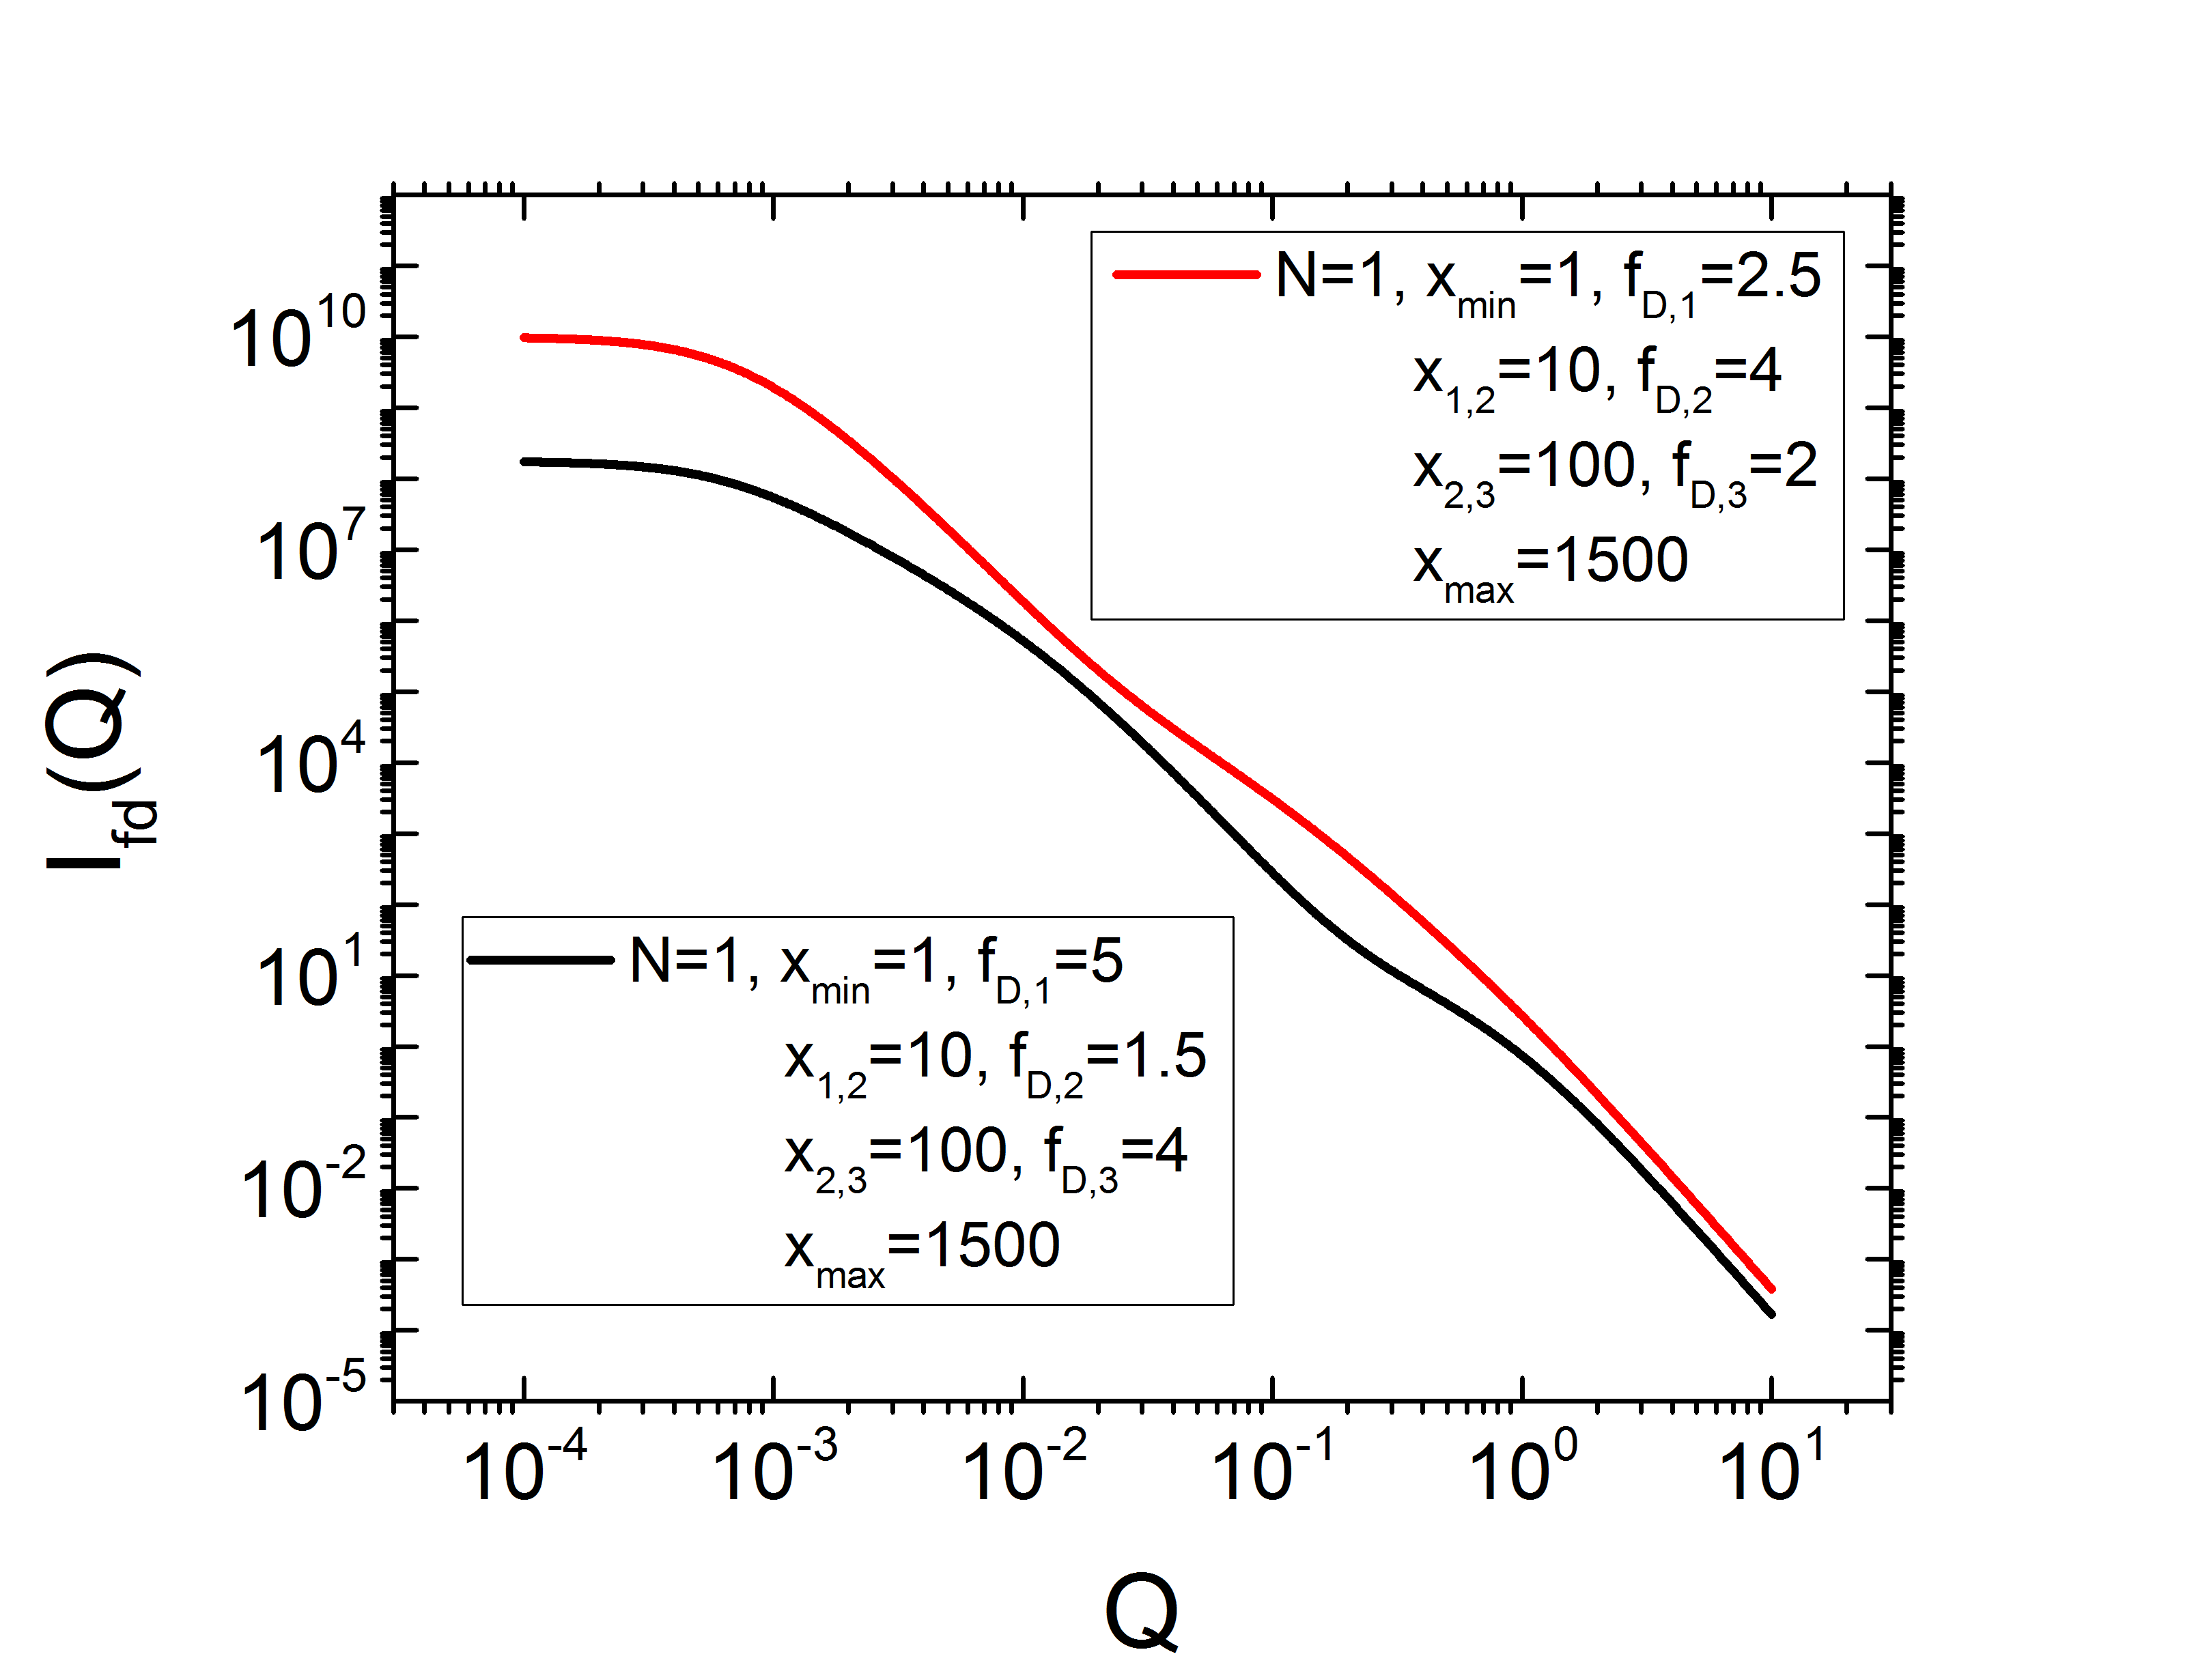
\includegraphics[width=0.47\textwidth]{../images/form_factor/fractal_series/fractalseries3IQ.png}}
  \quad
  \subfigure[fractal size distribution, the size distribution is zero for $x<x_\mathrm{min}$ and $x>x_\mathrm{max}$]{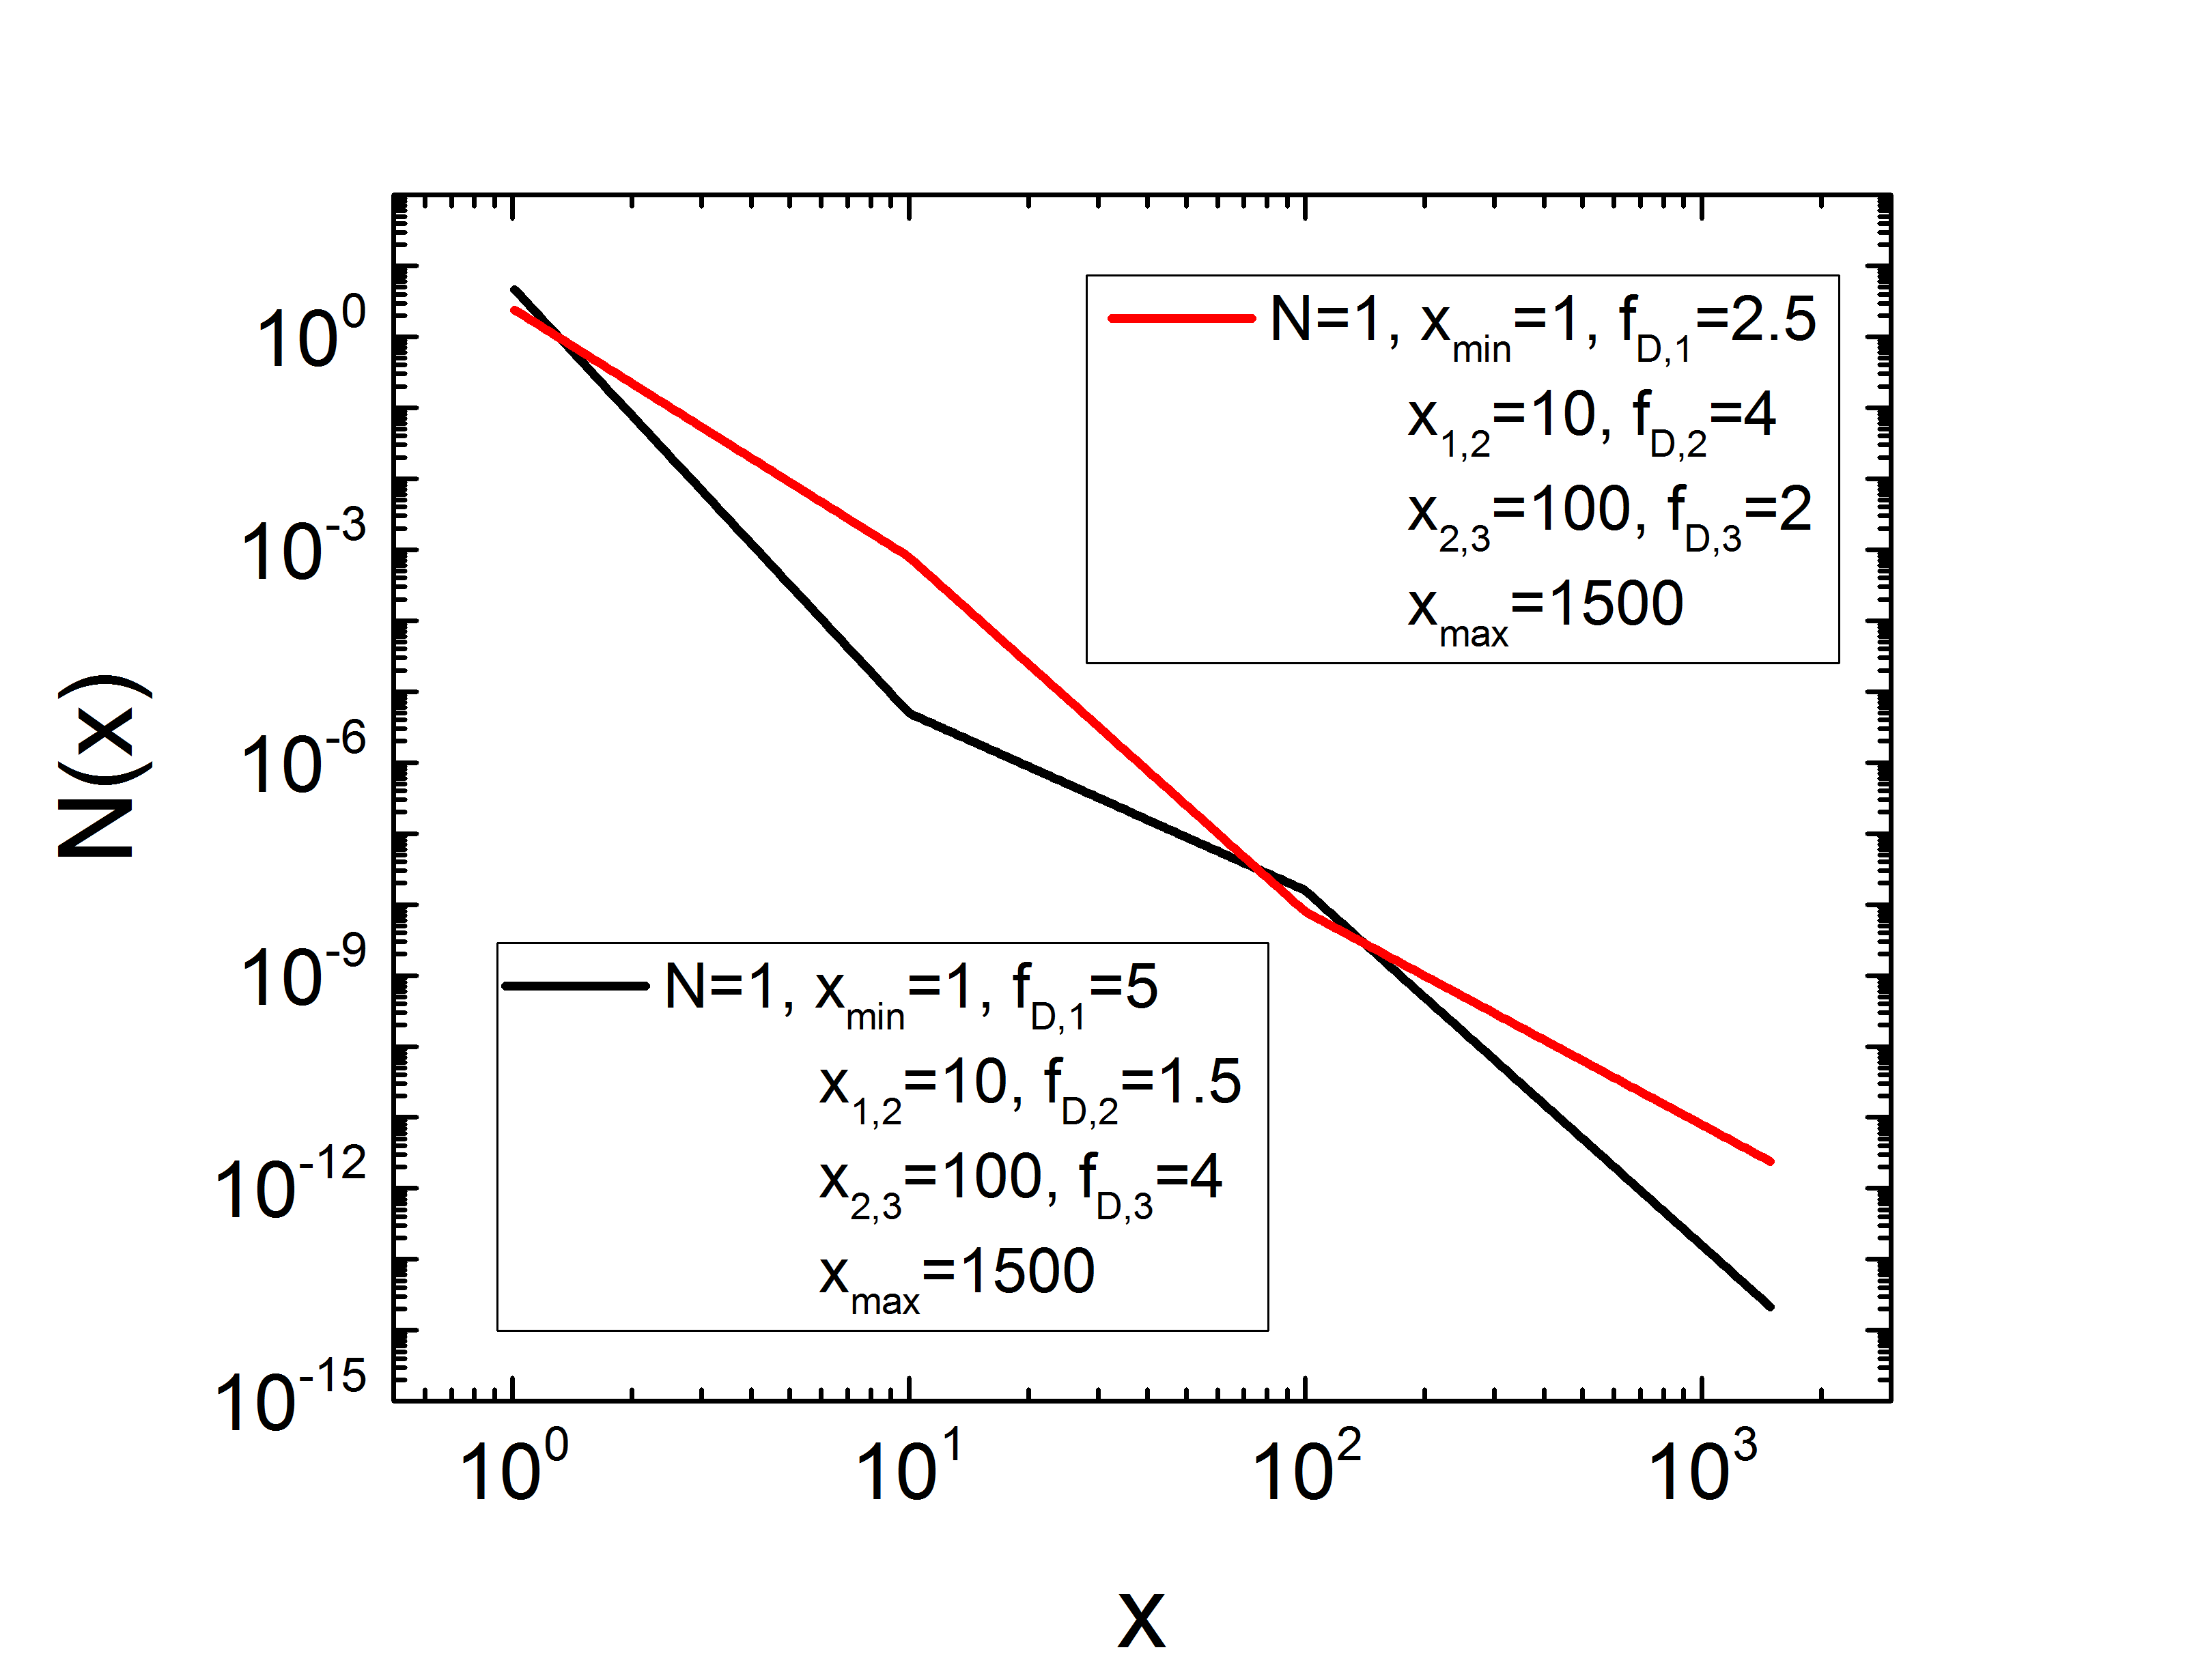
\includegraphics[width=0.47\textwidth]{../images/form_factor/fractal_series/fractalseries3Nx.png}}
  \label{fig:fractalseries}
  \caption{Scattering curve and corresponding size distribution for the plugin "\texttt{fractal series 3}".}
\end{figure}
